
\setcounter{chapter}{9}

\chapter{Flexible word meaning in embodied agents}
\label{c:flexible-grounded}
\label{c:gfwm}

In the previous chapter we demonstrated that word alignment strategies
which rely on competition between alternative word meaning hypotheses
are not applicable to embodied scenarios in which speakers and hearers
have substantially different perceptions of the objects in their
environment. As the final experiment of this thesis, we will now
tackle this problem by applying the flexible word representations from
Chapter \ref{c:flexible} to the robotic setup that we used in the last
3 chapters\footnote{Some parts of this chapter are adapted from
  \cite*{wellens08flexible}, see also
  \cite{wellens07flexible,wellens12multi-dimensional}}.


\begin{figure}[ht!] 
  
\parbox{\textwidth}{
  \renewcommand{\arraystretch}{1.3}
  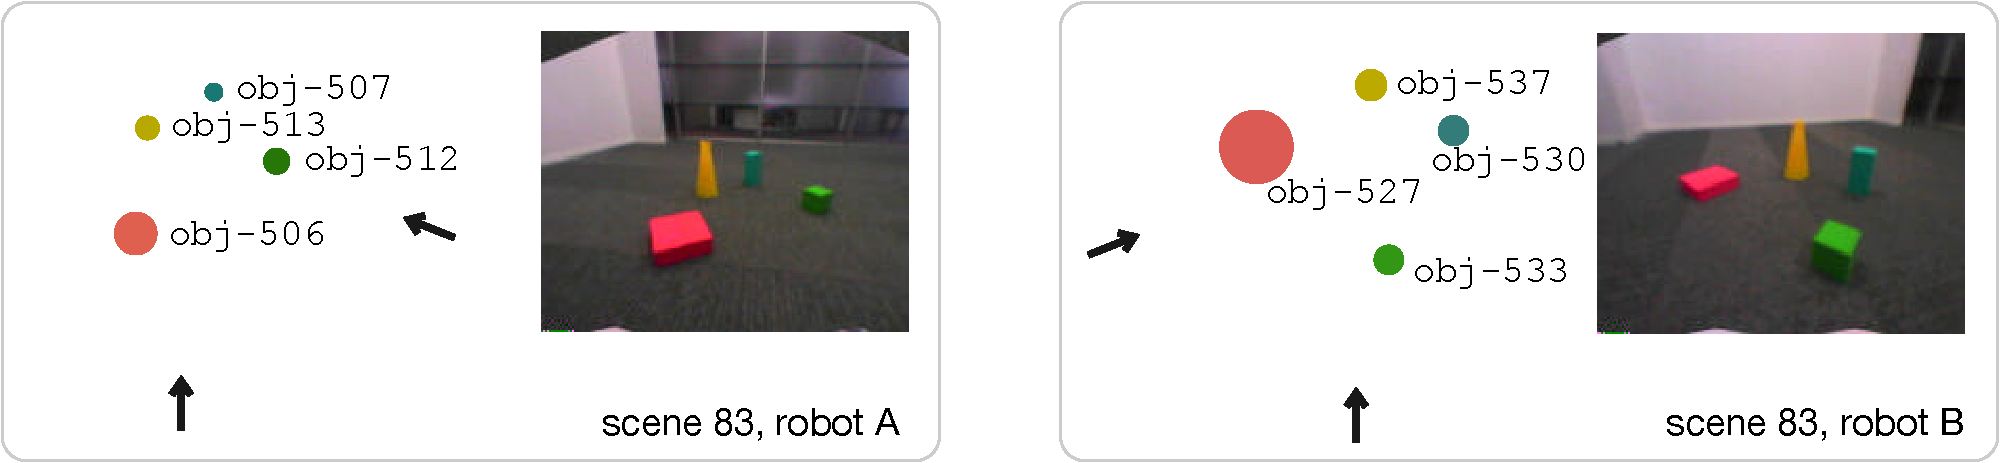
\includegraphics[width=1\textwidth]{figures/qfwm-example-world-models-scene-83}

  \vspace{0.3cm}
  \definecolor{dark}{rgb}{0.5,0.2,0}     
  
  \begin{center}
  \begin{tabular}{@{}ll}
    robot A &
    \begin{tabular}{@{}llll@{}}
      {\tt obj-512} & {\tt obj-507} & {\tt obj-513} & {\tt obj-506}  \\
      \hline
      \textcolor{dark}{\slshape x-3 } & { x-4 } & { x-4} & \textcolor{dark}{\slshape  x-2} \\
      \textcolor{dark}{\slshape y-1} & \textcolor{dark}{\slshape y-2} & \textcolor{dark}{\slshape y-3} & \textcolor{dark}{\slshape y-3} \\
      { width-2} & \textcolor{dark}{\slshape width-1} & { width-2} & \textcolor{dark}{\slshape width-3} \\
      \textcolor{dark}{\slshape height-2} & \textcolor{dark}{\slshape height-2} & { height-4} & { height-2} \\
      { luminance-2} & \textcolor{dark}{\slshape luminance-2} & { luminance-3} & { luminance-2} \\
      \textcolor{dark}{\slshape green-red-2} & { green-red-1} & { green-red-3} & { green-red-4} \\
      { yellow-blue-2} & { yellow-blue-3} & { yellow-blue-1} & \textcolor{dark}{\slshape yellow-blue-2} \\
      \hline
      
    \end{tabular}
  \end{tabular}
  
  \vskip0.5cm
  
  \begin{tabular}{@{}ll}
    robot B &
    \begin{tabular}{@{}llll@{}}
      {\tt obj-533} & {\tt obj-530} & {\tt obj-537} & {\tt obj-527} \\
      \hline
      \textcolor{dark}{\slshape  x-2} & {  x-4} & {  x-4} & \textcolor{dark}{\slshape  x-3} \\
      \textcolor{dark}{\slshape y-2} & \textcolor{dark}{\slshape y-1} & \textcolor{dark}{\slshape y-2} & \textcolor{dark}{\slshape y-4 }\\
      { width-2} & \textcolor{dark}{\slshape width-2} & { width-2} & \textcolor{dark}{\slshape width-4 }\\
      \textcolor{dark}{\slshape height-3} & \textcolor{dark}{\slshape height-3} & { height-4} & { height-2 }\\
      { luminance-2} & \textcolor{dark}{\slshape luminance-3} & { luminance-3} & { luminance-2 }\\
      \textcolor{dark}{\slshape green-red-1} & { green-red-1} & { green-red-3} & { green-red-4 }\\
      { yellow-blue-2} & { yellow-blue-3} & { yellow-blue-1} & \textcolor{dark}{\slshape yellow-blue-3}\\
      \hline
    
    \end{tabular}
  \end{tabular}
  \end{center}
  \vspace{0.2cm}}


%%% Local Variables: 
%%% mode: latex
%%% TeX-master: "../phdbook"
%%% End: 

  \caption{Interval based categorization. On the top, the an example
    scene as seen through the cameras of the two robots and the object
    models constructed by the vision system are shown. On the bottom,
    the categories that are applicable to each object are shown. Those
    categories that are different between the two robots are printed
    in italics.}
  \label{f:gfwm-scene}
\end{figure}

For comparability with the simulated version of this model, we assume
a categorization strategy that, similarly to discrimination trees,
splits sensory channels into four discrete regions. Agents are then
provided with sensory contexts that contain for each object all
applicable categories. An example of such sensory contexts from the
perspectives of two robots in a scene is shown in Figure
\ref{f:gfwm-scene}. As discussed in the previous chapter, perceptual
deviation inevitably causes both agents to categorize the same
physical objects differently, and indeed for all objects except the
yellow cone the applicable categories differ on four channels.


Everything else, i.e. the lexicon representation, the mechanisms for
production and interpretation, alignment strategies and even actual
parameters for certainty score updates and so on, are identical to the
experiments in Chapter \ref{c:flexible} (page \pageref{c:flexible}).


\section{Dealing with perceptual deviation}


\begin{figure}[p]
  
{\renewcommand{\arraystretch}{1.5}
\begin{tabular}{@{}p{0.95cm}|p{1.9cm}@{}p{0.6cm}@{}|p{1.9cm}@{}p{0.6cm}@{}|p{1.9cm}@{}p{0.6cm}@{}|p{1.9cm}@{}p{0.5cm}@{}}
form & agent 1 &  & agent 2 &  & agent 3 &  & agent 4 & \\
\hline
\textit{"weviwa"} & \texttt{green-red-2}

\texttt{yellow-blue-4}

\texttt{luminance-2}

\texttt{x-4}

\texttt{height-2} & 0.22

0.20

0.14

0.13

0.05 & \texttt{y-2}

\texttt{height-3}

\texttt{width-3}

\texttt{x-4}

\texttt{luminance-4}

\texttt{green-red-3}

\texttt{yellow-blue-1} & 0.13

0.13

0.04

0.02

0.02

0.02

0.02 & \texttt{height-2}

\texttt{green-red-2}

\texttt{yellow-blue-4}

\texttt{y-2} & 0.26

0.24

0.17

0.04 & \texttt{y-2}

\texttt{yellow-blue-4}

\texttt{luminance-2}

\texttt{green-red-2}

\texttt{height-2}

\texttt{x-3}

\texttt{y-4}

\texttt{height-3}

\texttt{luminance-1} & 0.17

0.13

0.10

0.10

0.08

0.02

0.02

0.02

0.02\\
\hline
\textit{"vumaza"} & \texttt{width-2}

\texttt{x-2}

\texttt{y-2}

\texttt{height-1}

\texttt{luminance-2}

\texttt{green-red-1}

\texttt{x-3}

\texttt{green-red-2}

\texttt{yellow-blue-4} & 0.26

0.17

0.17

0.17

0.13

0.06

0.02

0.02

0.02 & \texttt{width-2}

\texttt{luminance-2}

\texttt{x-3}

\texttt{y-4}

\texttt{height-2}

\texttt{green-red-3}

\texttt{yellow-blue-3}

\texttt{y-3}

\texttt{height-3}

\texttt{green-red-1}

\texttt{yellow-blue-4} & 0.30

0.14

0.10

0.10

0.10

0.10

0.10

0.06

0.02

0.02

0.02 & \texttt{y-3}

\texttt{green-red-4}

\texttt{width-2}

\texttt{yellow-blue-3} & 0.25

0.17

0.17

0.08 & \texttt{green-red-2}

\texttt{yellow-blue-4}

\texttt{width-2}

\texttt{x-2}

\texttt{y-2}

\texttt{y-3}

\texttt{width-1}

\texttt{height-2}

\texttt{luminance-2}

\texttt{x-3}

\texttt{height-3}

\texttt{luminance-3}

\texttt{green-red-1} & 0.14

0.14

0.14

0.10

0.10

0.10

0.10

0.10

0.10

0.02

0.02

0.02

0.02\\
\hline
\textit{"wedilo"} & \texttt{width-2}

\texttt{x-2}

\texttt{y-3}

\texttt{height-2}

\texttt{luminance-2}

\texttt{green-red-4}

\texttt{yellow-blue-3}

\texttt{y-2}

\texttt{x-3}

\texttt{height-3}

\texttt{luminance-3}

\texttt{green-red-1}

\texttt{yellow-blue-4} & 0.13

0.10

0.10

0.10

0.10

0.10

0.10

0.06

0.02

0.02

0.02

0.02

0.02 & \texttt{x-4}

\texttt{width-4}

\texttt{height-4}

\texttt{luminance-4}

\texttt{green-red-3}

\texttt{yellow-blue-1}

\texttt{yellow-blue-4} & 0.13

0.13

0.11

0.02

0.02

0.02

0.02 & \texttt{luminance-2}

\texttt{x-3}

\texttt{yellow-blue-3}

\texttt{y-4}

\texttt{width-2}

\texttt{height-3}

\texttt{luminance-3}

\texttt{green-red-3}

\texttt{yellow-blue-1}

\texttt{x-4}

\texttt{width-3} & 0.11

0.10

0.10

0.10

0.10

0.10

0.10

0.10

0.10

0.05

0.03 & \texttt{x-3}

\texttt{y-2} & 0.23

0.13\\
\hline
\textit{"lugefe"} & \texttt{luminance-2}

\texttt{x-4}

\texttt{yellow-blue-4} & 0.29

0.20

0.07 & \texttt{luminance-2}

\texttt{x-3}

\texttt{green-red-1}

\texttt{yellow-blue-3}

\texttt{height-3}

\texttt{yellow-blue-4} & 0.20

0.20

0.13

0.11

0.02

0.02 & \texttt{luminance-2}

\texttt{x-2}

\texttt{y-3}

\texttt{width-2}

\texttt{height-3}

\texttt{yellow-blue-3}

\texttt{green-red-4}

\texttt{x-3}

\texttt{width-1}

\texttt{height-2}

\texttt{green-red-2}

\texttt{yellow-blue-4} & 0.17

0.10

0.10

0.10

0.10

0.10

0.06

0.02

0.02

0.02

0.02

0.02 & \texttt{x-3}

\texttt{yellow-blue-4}

\texttt{y-1}

\texttt{width-3}

\texttt{height-4}

\texttt{green-red-1}

\texttt{luminance-2}

\texttt{y-3}

\texttt{width-2}

\texttt{height-2}

\texttt{luminance-1}

\texttt{green-red-2} & 0.13

0.13

0.10

0.10

0.10

0.10

0.06

0.06

0.02

0.02

0.02

0.02\\
\hline
\textit{"zubere"} & \texttt{y-2}

\texttt{yellow-blue-3}

\texttt{x-3}

\texttt{height-3}

\texttt{green-red-4} & 0.20

0.13

0.11

0.02

0.02 & \texttt{width-2}

\texttt{x-2}

\texttt{y-2}

\texttt{luminance-4}

\texttt{green-red-4}

\texttt{yellow-blue-3} & 0.20

0.20

0.10

0.10

0.10

0.10 & \texttt{x-2}

\texttt{y-3}

\texttt{luminance-3} & 0.17

0.17

0.07 & \texttt{x-2}

\texttt{yellow-blue-3} & 0.23

0.04
\end{tabular}}


%%% Local Variables: 
%%% mode: latex
%%% TeX-master: "../phdbook"
%%% End: 

  \caption{The meanings of the first five words of agent 1 (out of a
    population of 10 agents) and the corresponding categories in the
    lexicons of agents 2, 3 and 4 after 5000 interactions. The numbers
    right to the categories are scores of the association to the
    category.}
\label{f:gfwm-lexicon-forms-500}
\end{figure}

\begin{figure}[p]
  \rotatebox{90}
  {
\footnotesize\renewcommand{\arraystretch}{1.5}{
  \begin{tabular}{p{0.4cm}p{1.4cm}p{7cm}p{7cm}p{1.4cm}p{0.6cm}}
    \noalign{\vskip 0.5cm}\hskip 1cm
  \# & speaker + topic & word meanings speaker & word meanings hearer & hearer + topic & succ. \\
  \hline



2000 & agent 5 

\texttt{obj-7} &\textit{"kaloli"} (\texttt{luminance-2}\textsuperscript{.24}, \texttt{green-red-1}\textsuperscript{.19}, \texttt{yellow-blue-3}\textsuperscript{.03}, \texttt{width-2}\textsuperscript{.03}, \texttt{y-3}\textsuperscript{.02}, \texttt{width-1}\textsuperscript{.02}, \texttt{height-1}\textsuperscript{.02}, \texttt{luminance-4}\textsuperscript{.02})

\textit{"ketelu"} (\texttt{y-3}\textsuperscript{.28}, \texttt{luminance-2}\textsuperscript{.23}) & \textit{"kaloli"} (\texttt{luminance-2}\textsuperscript{.45}, \texttt{height-3}\textsuperscript{.20}, \texttt{yellow-blue-3}\textsuperscript{.18})

\textit{"ketelu"} (\texttt{luminance-2}\textsuperscript{.05}, \texttt{yellow-blue-4}\textsuperscript{.04}) & agent 7 

 \texttt{obj-8} & yes \\
2001 & agent 8 

\texttt{obj-17} &\textit{"xazafu"} (\texttt{green-red-3}\textsuperscript{.61}, \texttt{yellow-blue-1}\textsuperscript{.49})

\textit{"zisedu"} (\texttt{width-2}\textsuperscript{.36}, \texttt{y-3}\textsuperscript{.31}, \texttt{x-2}\textsuperscript{.22}) & \textit{"xazafu"} (\texttt{green-red-3}\textsuperscript{.49}, \texttt{yellow-blue-1}\textsuperscript{.42}, \texttt{luminance-4}\textsuperscript{.22}, \texttt{height-2}\textsuperscript{.15})

\textit{"zisedu"} (\texttt{y-2}\textsuperscript{.38}, \texttt{width-2}\textsuperscript{.22}, \texttt{yellow-blue-2}\textsuperscript{.07}) & agent 9 

 \texttt{obj-17} & yes \\
2002 & agent 4 

\texttt{obj-18} &\textit{"bekamo"} (\texttt{width-2}\textsuperscript{.41}, \texttt{green-red-4}\textsuperscript{.28}, \texttt{yellow-blue-2}\textsuperscript{.15}, \texttt{luminance-3}\textsuperscript{.14}, \texttt{y-2}\textsuperscript{.07}, \texttt{x-2}\textsuperscript{.05})

\textit{"pawegu"} (\texttt{x-3}\textsuperscript{.20}, \texttt{width-2}\textsuperscript{.17}, \texttt{luminance-2}\textsuperscript{.10}, \texttt{y-2}\textsuperscript{.09}) & \textit{"bekamo"} (\texttt{green-red-4}\textsuperscript{.44}, \texttt{width-2}\textsuperscript{.27}, \texttt{luminance-3}\textsuperscript{.25}, \texttt{yellow-blue-2}\textsuperscript{.23}, \texttt{y-2}\textsuperscript{.11}, \texttt{height-1}\textsuperscript{.03})

\textit{"pawegu"} (\texttt{height-2}\textsuperscript{.31}, \texttt{width-2}\textsuperscript{.15}) & agent 3 

 \texttt{obj-20} & yes \\
2003 & agent 1 

\texttt{obj-17} &\textit{"xazafu"} (\texttt{green-red-3}\textsuperscript{.49}, \texttt{yellow-blue-1}\textsuperscript{.43}, \texttt{luminance-4}\textsuperscript{.08}) & \textit{"xazafu"} (\texttt{green-red-3}\textsuperscript{.56}, \texttt{yellow-blue-1}\textsuperscript{.47}) & agent 6 

 \texttt{obj-17} & yes \\
2004 & agent 10 

\texttt{obj-100} &\textit{"bekamo"} (\texttt{green-red-4}\textsuperscript{.40}, \texttt{width-2}\textsuperscript{.27}, \texttt{luminance-3}\textsuperscript{.14}, \texttt{yellow-blue-2}\textsuperscript{.08}, \texttt{height-2}\textsuperscript{.05})

\textit{"pawegu"} (\texttt{y-2}\textsuperscript{.17}, \texttt{yellow-blue-3}\textsuperscript{.17}, \texttt{x-4}\textsuperscript{.10}, \texttt{width-3}\textsuperscript{.10}, \texttt{height-3}\textsuperscript{.10}, \texttt{luminance-2}\textsuperscript{.10}, \texttt{green-red-1}\textsuperscript{.10}, \texttt{yellow-blue-2}\textsuperscript{.10}, \texttt{x-3}\textsuperscript{.05}, \texttt{green-red-4}\textsuperscript{.05})

\textit{"xivima"} (\texttt{luminance-2}\textsuperscript{.40}, \texttt{yellow-blue-3}\textsuperscript{.35}, \texttt{x-3}\textsuperscript{.06}, \texttt{width-3}\textsuperscript{.06}, \texttt{height-3}\textsuperscript{.06}, \texttt{green-red-4}\textsuperscript{.06}) & \textit{"bekamo"} (\texttt{x-2}\textsuperscript{.28}, \texttt{yellow-blue-2}\textsuperscript{.27}, \texttt{width-2}\textsuperscript{.24}, \texttt{green-red-4}\textsuperscript{.13}, \texttt{y-3}\textsuperscript{.10}, \texttt{luminance-3}\textsuperscript{.10})

\textit{"pawegu"} (\texttt{x-4}\textsuperscript{.13}, \texttt{width-3}\textsuperscript{.13}, \texttt{height-3}\textsuperscript{.13}, \texttt{y-2}\textsuperscript{.13}, \texttt{x-2}\textsuperscript{.03}, \texttt{luminance-2}\textsuperscript{.02}, \texttt{yellow-blue-2}\textsuperscript{.02})

\textit{"xivima"} (\texttt{luminance-2}\textsuperscript{.41}, \texttt{yellow-blue-3}\textsuperscript{.26}, \texttt{y-3}\textsuperscript{.13}, \texttt{green-red-4}\textsuperscript{.13}, \texttt{height-3}\textsuperscript{.06}, \texttt{x-2}\textsuperscript{.02}, \texttt{height-2}\textsuperscript{.02}, \texttt{green-red-1}\textsuperscript{.02}) & agent 8 

 \texttt{obj-99} & yes \\
2005 & agent 3 

\texttt{obj-17} &\textit{"xazafu"} (\texttt{green-red-3}\textsuperscript{.65}, \texttt{yellow-blue-1}\textsuperscript{.54}, \texttt{luminance-4}\textsuperscript{.24}) & \textit{"xazafu"} (\texttt{green-red-3}\textsuperscript{.49}, \texttt{yellow-blue-1}\textsuperscript{.43}, \texttt{luminance-4}\textsuperscript{.24}, \texttt{height-2}\textsuperscript{.11}) & agent 9 

 \texttt{obj-17} & yes \\
2006 & agent 4 

\texttt{obj-109} &\textit{"xazafu"} (\texttt{green-red-3}\textsuperscript{.49}, \texttt{yellow-blue-1}\textsuperscript{.43}, \texttt{luminance-4}\textsuperscript{.22}) & \textit{"xazafu"} (\texttt{green-red-3}\textsuperscript{.50}, \texttt{yellow-blue-1}\textsuperscript{.44}, \texttt{luminance-4}\textsuperscript{.09}) & agent 1 

 \texttt{obj-109} & yes \\
2007 & agent 5 

\texttt{obj-81} &\textit{"pokosa"} (\texttt{height-2}\textsuperscript{.26}, \texttt{x-2}\textsuperscript{.22}, \texttt{y-4}\textsuperscript{.10}, \texttt{width-2}\textsuperscript{.10}, \texttt{height-3}\textsuperscript{.10}, \texttt{green-red-2}\textsuperscript{.10})

\textit{"doteza"} (\texttt{y-2}\textsuperscript{.26}, \texttt{width-2}\textsuperscript{.19}, \texttt{x-3}\textsuperscript{.17}) & \textit{"pokosa"} (\texttt{yellow-blue-3}\textsuperscript{.27}, \texttt{green-red-1}\textsuperscript{.17}, \texttt{width-2}\textsuperscript{.15}, \texttt{y-2}\textsuperscript{.11}, \texttt{height-3}\textsuperscript{.10}, \texttt{x-2}\textsuperscript{.07})

\textit{"doteza"} (\texttt{green-red-1}\textsuperscript{.13}, \texttt{x-3}\textsuperscript{.13}, \texttt{height-1}\textsuperscript{.13}, \texttt{y-3}\textsuperscript{.10}, \texttt{luminance-3}\textsuperscript{.10}, \texttt{yellow-blue-2}\textsuperscript{.06}, \texttt{y-2}\textsuperscript{.02}, \texttt{width-1}\textsuperscript{.02}, \texttt{luminance-4}\textsuperscript{.02}, \texttt{yellow-blue-3}\textsuperscript{.02}) & agent 8 

 \texttt{obj-81} & yes \\
2008 & agent 2 

\texttt{obj-152} &\textit{"xazafu"} (\texttt{green-red-3}\textsuperscript{.48}, \texttt{yellow-blue-1}\textsuperscript{.48}) & \textit{"xazafu"} (\texttt{green-red-3}\textsuperscript{.62}, \texttt{yellow-blue-1}\textsuperscript{.49}) & agent 8 

 \texttt{obj-148} & yes \\
2009 & agent 1 

\texttt{obj-104} &\textit{"regowo"} (\texttt{yellow-blue-4}\textsuperscript{.44}, \texttt{green-red-2}\textsuperscript{.40}) & \textit{"regowo"} (\texttt{yellow-blue-4}\textsuperscript{.28}, \texttt{y-3}\textsuperscript{.22}, \texttt{green-red-2}\textsuperscript{.19}) & agent 5 

 \texttt{obj-107} & yes \\


\noalign{\vskip 1cm}   
\end{tabular}}}
  \caption{Overview of 10 consecutive interactions in a population of
    10 agents from game 2000 on. It shows the speaker with his chosen
    topic, the words used by the speaker with their associated
    meanings (the association scores are in superscript), the word
    meanings interpreted by the hearer, the hearer and the interpreted
    topic, and whether the agents reached communicative success.}
  \label{f:gfwm-trace}
\end{figure}


With flexible word representations, agents do not try trying to find
the ``correct'' mapping from a form to a meaning among a set of
competing hypothesis, but rather capture the uncertainty how to
conceptualize objects in the word representations themselves. Figure
\ref{f:gfwm-lexicon-forms-500} shows a partial snapshot of the early
lexicons of four agents after 500 interactions. Although there is some
initial coherence, very different categories are associated to each
form by different agents, very often even from the same sensory
channel.



Nevertheless, as already discussed in Chapter \ref{c:flexible}, agents
are able to use these highly un-conventionalized word meanings
successfully from very early on, because the similarity based lexicon
application does not require all categories of a meaning to be
applicable to the topic -- it is enough that the similarity of the
words of the utterance to the topic is highest compared to the all
other objects in the context. This is illustrated in Figure
\ref{f:gfwm-trace}, which lists 10 consecutive language games from
interaction 2000 on. All of these interactions succeed, although the
category sets that speaker and hearer connect to the words in the
utterance are often very different. Furthermore (as we already
observed in non-grounded version), using multi-word utterances does
not increase the risk of communicative failure but rather decreases
it, because the likelihood of finding the right topic is the higher
the more (partially conventionalized) words are used in the
similarity-based lexicon application.

\begin{figure}[t]
  
{\renewcommand{\arraystretch}{1.5}
\begin{tabular}{@{}p{0.95cm}|p{1.9cm}@{}p{0.6cm}@{}|p{1.9cm}@{}p{0.6cm}@{}|p{1.9cm}@{}p{0.6cm}@{}|p{1.9cm}@{}p{0.5cm}@{}}
form & agent 1 &  & agent 2 &  & agent 3 &  & agent 4 & \\
\hline
\textit{"weviwa"} & \texttt{yellow-blue-4}

\texttt{green-red-2} & 0.74

0.53 & \texttt{yellow-blue-4}

\texttt{green-red-2} & 0.73

0.55 & \texttt{yellow-blue-4}

\texttt{green-red-2} & 0.68

0.38 & \texttt{yellow-blue-4}

\texttt{green-red-2} & 0.70

0.58\\
\hline
\textit{"vumaza"} & \texttt{yellow-blue-3}

\texttt{width-2} & 0.35

0.17 & \texttt{width-2}

\texttt{x-2}

\texttt{y-2}

\texttt{yellow-blue-2}

\texttt{luminance-2}

\texttt{green-red-1} & 0.21

0.09

0.06

0.06

0.02

0.02 & \texttt{x-2}

\texttt{y-3}

\texttt{width-2} & 0.34

0.32

0.18 & \texttt{width-2}

\texttt{x-2}

\texttt{y-3}

\texttt{luminance-2} & 0.46

0.19

0.08

0.06\\
\hline
\textit{"wedilo"} & \texttt{yellow-blue-3}

\texttt{green-red-4}

\texttt{luminance-2}

\texttt{y-2}

\texttt{width-3} & 0.70

0.62

0.38

0.04

0.04 & \texttt{yellow-blue-3}

\texttt{green-red-4}

\texttt{luminance-2} & 0.68

0.54

0.43 & \texttt{yellow-blue-3}

\texttt{green-red-4}

\texttt{luminance-2} & 0.67

0.50

0.41 & \texttt{yellow-blue-3}

\texttt{green-red-4}

\texttt{luminance-2} & 0.68

0.53

0.43\\
\hline
\textit{"lugefe"} & \texttt{luminance-2} & 0.55 & \texttt{luminance-2}

\texttt{width-2} & 0.59

0.21 & \texttt{luminance-2}

\texttt{green-red-1}

\texttt{y-3} & 0.51

0.22

0.03 & \texttt{luminance-2}

\texttt{y-3} & 0.43

0.06\\
\hline
\textit{"zubere"} & \texttt{height-2}

\texttt{width-2}

\texttt{y-2} & 0.34

0.17

0.04 & \texttt{height-2}

\texttt{width-2}

\texttt{x-2} & 0.55

0.07

0.07 & \texttt{height-2}

\texttt{width-2}

\texttt{y-2} & 0.35

0.22

0.21 & \texttt{height-2}

\texttt{width-2}

\texttt{x-2} & 0.55

0.21

0.08
\end{tabular}}

%%% Local Variables: 
%%% mode: latex
%%% TeX-master: "../phdbook"
%%% End: 

  \caption{Meanings of the same words as in Figure
    \ref{f:gfwm-lexicon-forms-500} at interaction 10000. }
  \label{f:gfwm-lexicon-forms-10000}
\end{figure}


\begin{figure}[t]
  \gnuplotfigure{figures/gfwm-channel-entrenchment}
  \caption{Success of categories in communication per sensory channel.
    For all categories of the first agent in the population, the
    average association scores to the connected forms are plotted per
    channel along the x axis.}
  \label{f:gfwm-channel-entrenchment}
\end{figure}


\begin{figure}[t]
  \centerline{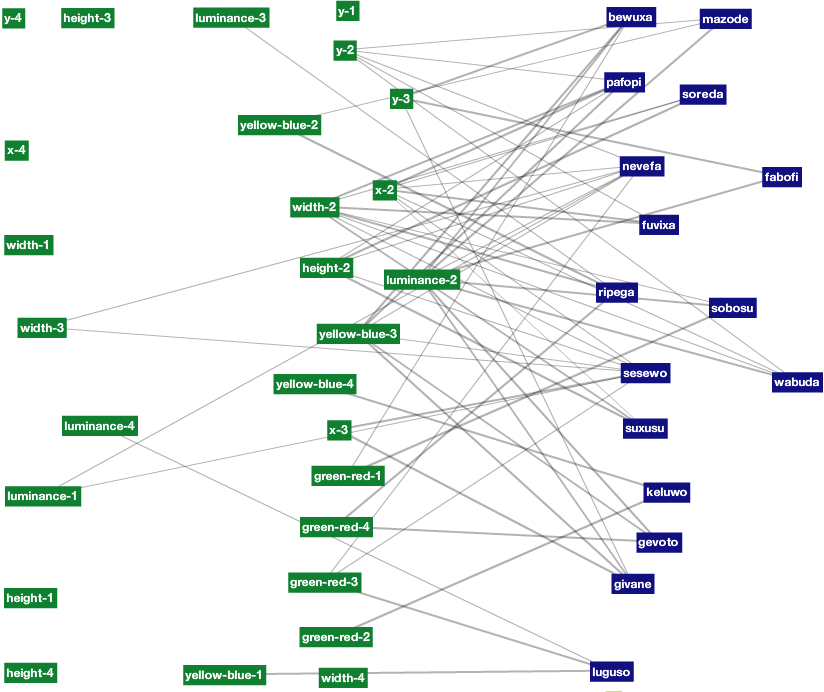
\includegraphics[width=0.8\textwidth]{figures/gfwm-lexicon-20000}}
  \caption{Network visualization of the he lexicon of the first agent
    of the population after 20000 interactions. For each word form,
    all categories that are associated to the form are shown. Line
    width denote association weights.}
  \label{f:gfwm-semiotic-network-example}
\end{figure}

Carefully shaping these categories in subsequent interactions, agents
reach high coherence in their lexicons. Figure
\ref{f:gfwm-lexicon-forms-10000} shows the lexicons of the same agents
9500 interactions later, and it turns all first five words from
interaction 500 survived in the lexicons of all the agents, and a
consensus on a core set of categories has been reached. Furthermore,
the aligned lexicons contain words of different degrees of specificity
(unlike the competition based lexicon formation models, which had a
bias towards atomic word meanings) -- the lexicons in Figure
\ref{f:gfwm-lexicon-forms-10000} contain both very general and very
specific words. As an example for a general word, ``lugefe'' is
consistently associated to the single category \texttt{luminance-2},
which makes it applicable to all ``dark'' objects. In contrast,
``wedilo'' is an example for a very specific word, it is associated by
all four agents to the tree categories \texttt{yellow-blue-3},
\texttt{green-red-4} and \texttt{luminance-2}, which makes the word
only applicable to dark purple or pink objects. In between, words such
as ``weviwa'' (``turquoise'') or ``zubere'' (``small'') cover two
categories.


Note that categories on channels such as \texttt{yellow-blue} and
\texttt{green-red} have higher association scores than others.
Similarly to the experiments in the previous two chapters, agents rely
more on categories on channels with smaller perceptual deviation,
which is further illustrated in Figure
\ref{f:gfwm-channel-entrenchment}. The average association scores
between forms and categories are highest for categories on the
\texttt{yellow-blue}, \texttt{luminance} and \texttt{green-red}
channels, which again matches their observed correlations across all
the perceptions of both robots (see Figure
\ref{f:data-sets-perceptual-deviation-matrix} on page
\pageref{f:data-sets-perceptual-deviation-matrix}). Furthermore, some
categories on channels with higher perceptual deviation end up being
removed from all the words in the lexicon, as shown in Figure
\ref{f:gfwm-semiotic-network-example}.




\startfiguregroup

\begin{figure}[t]
  \gnuplotfigure{figures/qfwm-attribute-scores-1}
  \caption{Example of the evolution of a single word of a single agent
    over time (interactions). Along the x-axis, the association scores
    to each category of the word are plotted.}
\label{f:qfwm-attribute-scores-1}
\end{figure}

\begin{figure}[t]
  \gnuplotfigure{figures/qfwm-attribute-scores-2}
  \caption{Example of the evolution of a second word over time.}
  \label{f:qfwm-attribute-scores-2}
\end{figure}

\begin{figure}[t]
  \gnuplotfigure{figures/qfwm-attribute-scores-3}
  \caption{Example of the evolution of a third word over time.}
  \label{f:qfwm-attribute-scores-3}
\end{figure}

\begin{figure}[t]
  \gnuplotfigure{figures/qfwm-attribute-scores-4}
  \caption{Example of the evolution of a fourth word over time.}
  \label{f:qfwm-attribute-scores-4}
\end{figure}

\stopfiguregroup

~\\

Finally, Figures
\ref{f:qfwm-attribute-scores-1}--\ref{f:qfwm-attribute-scores-4}
provide four examples of the changing association of word forms to
different categories, demonstrating the capability to gradually shift
word meanings in order to make them more applicable to the objects in
the world. A word that constantly changes its dominant meaning is
shown in Figure
\ref{f:qfwm-attribute-scores-1}. It is invented
or adopted at around interaction 6000 and subsequently undergoes many
meaning shifts.  Over time, the highest association scores are to {\tt
  height-3} (interaction 7000), {\tt yellow-blue-2} (interaction
16000), {\tt width-2} (21000 - 36000) and {\tt luminance-2} (40000).
In addition to that, many other categories are associated with the
word, but are immediately discarded again. The situation stabilizes
towards the end, giving the word the final meaning ``narrow, dark,
yellow''.  In contrast, Figure
\ref{f:qfwm-attribute-scores-2} is an example of
a rather unsuccessful word. The initial meanings disappear quite soon
and at around interaction 5000, a stable set of three categories
arises. This meaning does not seem to spread and the word loses all
its categories after 22000 interactions.  Thereafter the agent does
not use the word himself in production, but other agents in the
population still use it, leading to new associations with categories,
which eventually also don't turn out to be successful.

An example for a word that changes from being very specific to very
general is shown in Figure
\ref{f:qfwm-attribute-scores-3}. Except for some
quickly disappearing other associations, this word is initially only
connected to {\tt width-2}.  Over the course of more interactions,
more and more categories are associated ({\tt luminance-3} at around
interaction 3000, {\tt green-red-4} at interaction 7000 and finally
{\tt height-2} at interaction 22000).  So this word changed from being
very general (``thin'') to very specific (``thin, low, bright and
red''). In contrast, the word in Figure
\ref{f:qfwm-attribute-scores-4} is an example of
the opposite. It starts being very specific, with connections to {\tt
  green-red-4}, {\tt yellow-blue-2}, {\tt height-2}, {\tt width-2},
{\tt luminance-3} (``orange, small and bright'').  It looses most of
its categories, becoming very general (``orange'') towards the end.



\section{Success without coherence}


\begin{figure}[t]
  \gnuplotfigure{figures/gfwm-success+lexicon-size+coherence}
  \caption{Comm\-unicative success (measure
    \ref{m:communicative-success}), lexicon size (measure
    \ref{m:lexicon-size}) and lexicon coherence (measure
    \ref{m:fwm-lexicon-coherence}) in a population of 10 agents
    averaged over 10 repeated series of 20000 language games.}
  \label{f:gfwm-success+lexicon-size+coherence}
\end{figure}


Throughout this thesis, the flexible word representations and
alignment strategies are the only lexicon formation model that could
be applied without modification to a setup with physical robots in a
real world. Figure \ref{f:gfwm-success+lexicon-size+coherence} shows
the overall alignment dynamics, which look very similar to the
non-grounded version (Figure
\ref{f:sfwm-success+lexicon-size+coherence} on page
\pageref{f:sfwm-success+lexicon-size+coherence}). Already after a few
hundred interactions agents communicate successfully in more than 50\%
of the cases, and by further extending and refining their lexicons
agents reach about 90\% communicative success, which is remarkably
high for grounded language games. Even more so than in the
non-grounded version, lexicon coherence is not a prerequisite for
communicative success -- it is even below zero in the first 2000
interaction (due to it's computation using the set similarity measure)
and grows only slowly later on. This again shows that the similarity
based lexicon application allows agents to stretch their initial word
meanings to broad use cases and thus allows them to communicate
successfully.


\begin{figure}[t]
  \gnuplotfigure{figures/gfwm-lexicon}
  \caption{The distance of the utterance to the topic (measure
    \ref{m:fwm-distance-utterance-topic}), the average number of
    categories covered per word (measure
    \ref{m:fwm-attributes-per-word}) and the average utterance length
    (measure \ref{m:utterance-length}) are averaged over 10 repeated
    series of 20000 language games.}
  \label{f:gfwm-lexicon}
\end{figure}


Furthermore, the word usage dynamics (Figure \ref{f:gfwm-lexicon})
look almost identical to their non-grounded counterpart (Figure
\ref{f:sfwm-lexicon} on page \pageref{f:sfwm-lexicon}). The distance
between the words of the utterance and the topic quickly decreases,
and on average two words that cover on average 4 categories are part
of each utterance.

\startfiguregroup


\begin{figure}[t]
  \gnuplotfigure{figures/gfwm-communicative-success-vs-population-size}
  \caption{Communi\-cative success (measure
    \ref{m:communicative-success}) for five different population
    sizes. Results are averaged over 10 series of varying length, but
    each with 8000 interactions per agent.}
  \label{f:gfwm-communicative-success-vs-population-size}
\end{figure}

\begin{figure}[t]
  \gnuplotfigure{figures/gfwm-lexicon-size-vs-population-size}
  \caption{Lexicon size (measure \ref{m:lexicon-size}) for five
    different population sizes. Results are averaged over 10 series of
    varying length, but each with 8000 interactions per agent.}
  \label{f:gfwm-lexicon-size-vs-population-size}
\end{figure}

\begin{figure}[t]
  \gnuplotfigure{figures/gfwm-lexicon-coherence-vs-population-size}
  \caption{Lexicon coherence (measure \ref{m:fwm-lexicon-coherence})
    for five different population sizes. Results are averaged over 10
    series of varying length, but each with 8000 interactions per
    agent.}
  \label{f:gfwm-lexicon-coherence-vs-population-size}
\end{figure}

\stopfiguregroup

~\\

Finally, Figures
\ref{f:gfwm-communicative-success-vs-population-size}--\ref{f:gfwm-lexicon-coherence-vs-population-size}
investigate the scaling with population size and it shows that the
model scales even slightly better with increasing population sizes
than the non-grounded version (compare page
\pageref{f:gfwm-communicative-success-vs-population-size}). Without
having looked into it, we speculate that this is because the physical
world of our robots is more structured than the simulate world, which
provides an external structure for the word meanings and thus makes
the alignment task easier.
 




%%% Local Variables: 
%%% mode: latex
%%% TeX-master: "phd-thesis"
%%% End: 
